

\documentclass[paper=a4, fontsize=11pt]{scrartcl} % A4 paper and 11pt font size

\usepackage[T1]{fontenc} % Use 8-bit encoding that has 256 glyphs
\usepackage{fourier} % Use the Adobe Utopia font for the document - comment this line to return to the LaTeX default
\usepackage[english]{babel} % English language/hyphenation
\usepackage{amsmath,amsfonts,amsthm} % Math packages
\usepackage{bm}
\usepackage{graphicx}
\usepackage{lipsum} % Used for inserting dummy 'Lorem ipsum' text into the template
\usepackage{mathtools}
\usepackage{caption}
\usepackage{subcaption}
\usepackage{color}
\usepackage{sectsty} % Allows customizing section commands
\allsectionsfont{\centering \normalfont\scshape} % Make all sections centered, the default font and small caps

\usepackage{fancyhdr} % Custom headers and footers
\pagestyle{fancyplain} % Makes all pages in the document conform to the custom headers and footers
\fancyhead{} % No page header - if you want one, create it in the same way as the footers below
\fancyfoot[L]{} % Empty left footer
\fancyfoot[C]{} % Empty center footer
\fancyfoot[R]{\thepage} % Page numbering for right footer
\renewcommand{\headrulewidth}{0pt} % Remove header underlines
\renewcommand{\footrulewidth}{0pt} % Remove footer underlines
\setlength{\headheight}{13.6pt} % Customize the height of the header

\numberwithin{equation}{section} % Number equations within sections (i.e. 1.1, 1.2, 2.1, 2.2 instead of 1, 2, 3, 4)
\numberwithin{figure}{section} % Number figures within sections (i.e. 1.1, 1.2, 2.1, 2.2 instead of 1, 2, 3, 4)
\numberwithin{table}{section} % Number tables within sections (i.e. 1.1, 1.2, 2.1, 2.2 instead of 1, 2, 3, 4)

\setlength\parindent{0pt} % Removes all indentation from paragraphs - comment this line for an assignment with lots of text

\title{LTV prediction using probabilistic models}
\author{Jonatan Pi\~nol and Peter Weber}
\date{} % delete this line to display the current date

%%% BEGIN DOCUMENT
\begin{document}

\maketitle
\tableofcontents

\newpage
\section{Introduction}

In this project we want to perform an estimation of customer life-time value (LTV) as a case of a Customer-Base Analysis using what literature in this domain calls probabilistic models, which is in reality no other thing than using a Bayesian approach. We will be using two datasets from the company where we work.

This work will be divided in the following parts: First, a discussion of Customer-Basis Analysis and possible scenarios and characterization of our scenario. Second, a description of the model we will use (assumptions etc...), and, third, a discussion about implementation of the model. Finally, we will present the results obtained and a short evaluation of the model.

We found that this would make a proper project for a "Bayesian Statistics" course, as it is in between a Data-oriented and an Application-oriented project type.

\section{Customer Basis Analysis}

Customer Basis Analysis is a concept that is being more and more critical as companies have access (or generate) to more customer's transaction data (increase in complexity and volume). The avaibility of these datasets has lead to a general change from transaction based strategies to more customer-centric strategies. In other words, the first strategies lead typically to descriptive analysis (for example summary statistic like rates, average number of subscriptions ...), while the customer-centric approach is more focused on analysis on the user behaviour which forms the basis for a more predictive approach. Using characteristics and past behaviour (found in those databases) a forecast can be made. This is why a Bayesian Probabilistic approach can be convenient.

\subsection{Probabilistic models for Customer Basis Analysis}

As usual for a probabilistic model, the problem will be modeled in a way that observed behavior has an underlying random process. Thus, past behavior is not a true mirror of future actions. With this interpretation, the past, and the "future" are function of latent characteristics denoted by $\theta$ .

While this approach may not be new (in other fields), the novelty resides in the fact that classically for Customer Basis Analysis, the approaches have been regression-like (which also happened in the company we work) and the use of probabilistic approaches is relatively new.

\subsection{Possible scenarios:}

Commonly in literature we will find the following classification for scenarios in Customer-Base Analysis, which is shown in Fig.~\ref{fig:Relation}.
First we have, by opportunities of transactions. It can be discrete and continuous. Second, by relation with the customer. Here, the key distinction between contractual and noncontractual is that in a contractual scenario, one observes when a customer leaves, while in a noncontractual scenario, a customer's departure is unobservable and therefore must be inferred. For example, in a contractual scenario, a user might pay for a service only when needed, so that if during a long time this user didn't make any transaction either it should be considered that he not any more a client or it's just a hiatus, we don't know it directly.

\begin{figure}[h!]
\centering
  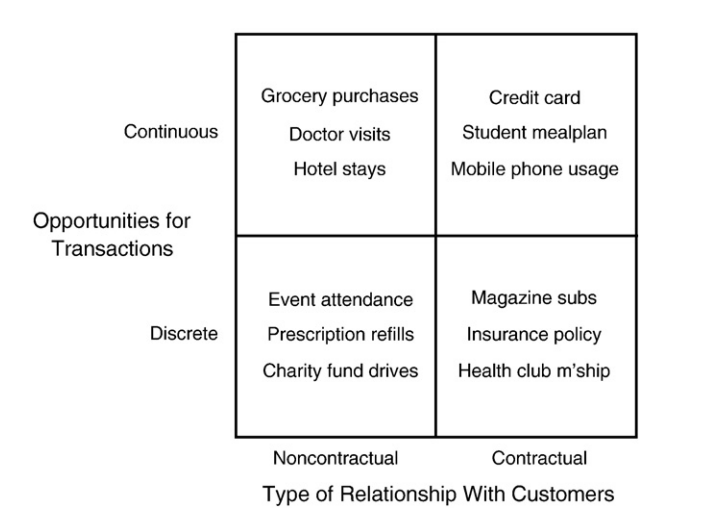
\includegraphics[scale = 0.75]{CustomerRelation.png}
  \caption{Examples for the different scenarios. From \cite{fader09} }
  \label{fig:Relation}
\end{figure}

The company in which we work, has a few subscription based websites, where users are subscrived in order to have access to contents and services. After each cycle (30 days) the user is automatically rebilled and in order to drop out, the user has to cancel his subscription. This scenario corresponds to a contractual scenario where transactions are done periodically.

Concretely, we will work with data from two products, which underly the same type of setting but slightly different user behaviour.

\subsection{Our case: Model LTV prediction}
For the scope of this project, we will model the Customer Life Time Value as a particular case of Customer Basis Analysis, using a Bayesian Probabilistic model.

In marketing, customer lifetime value (CLV or often CLTV), or life-time value (LTV) is a prediction of the net revenue attributed to the entire future relationship with a customer. The prediction model can have varying levels of sophistication and accuracy, ranging from a crude heuristic to the use of complex predictive analytics techniques. Many businesses strongly depend on this metric as it is their only projection of revenue for the near future.

For this, we will implement the proposed model for Customer Retention Prediction described in \cite{fader07}, on our datasets.

\section{Dataset description}

 Our case is of a Discrete Contractual scenario (as we see in \ref{fig:Relation}) , with a 30 days period cycle of rebill. The users can cancel their relation with the company at any time.
 The data we use has been collected over the last two years and it is composed of number of clients that rebill after each cycle. We have added two additional columns that will be useful for modeling, the number of clients as a percentage and the number of users that cancels during each cycle. In particular, we start off with about 47 thousand users that initially sign up, and then on every cycle we loose some of these users. We consider 12 rebill cycles in total. The second dataset looks similar. Both datasets will be provided as .rds files, which are read in by the provided R file.

 \begin{figure}[h!]
 	\centering
  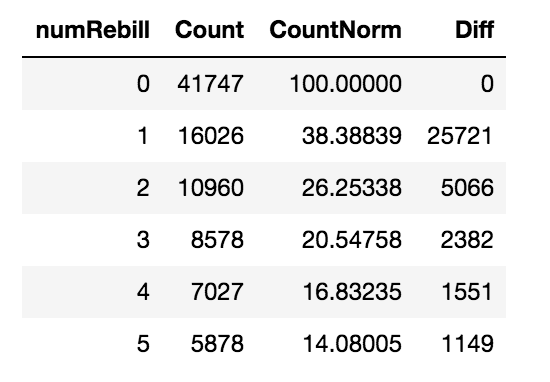
\includegraphics[scale = 0.55]{Data_sample.png}
  \caption{Number of user rebilling at each cycle}
  \label{fig:Data_sample}
\end{figure}

\section{Model: Shifted Geometrical Beta distribution for retention prediction}
 
 Our first idea to approach this problem was using a Negative Binomial with a Beta distribution as prior. We first tried this implementation with an MCMC implementation in order to estimate the probability of cancel of the users. For this model to be applicable we always need data of the full customer lifetime, as we only model the cancellation of users. In this approach all users should be cancelled after the last rebilling cycle that is considered.
 
 However, as we want to use this model to predict the full customer lifetime, but having only a few rebill cycles for the user we need a model that takes into account the users that are still active at the end of our observation period. This is exactly what the model presented in \cite{feder07} considers. Therefore, we will implement their approach and apply it to our data.
 
 The model we want to test is also based on using a negative binomial distribution (more precisely a geometric distribution as the failure number $r$ is set to 1), with an additional term that enables to consider the surviving users. Let's see this model in more detail. 
 
 \subsection{Model Assumptions} 
 The assumptions of the model are:
 \begin{itemize}
  \item At the end of each cylce, the user renews its subscription or cancels with some probability
  \item That probability remains constant for every user, but
  \item is heterogeneous accross users.
\end{itemize}
 
 Those assumptions are translated in the following probabilities. The probability of duration for a given user( we will call it retention function), in terms of counts of rebills (success) before cancel the contract (failure), which is a classical Negative Binomial Distributio with $r=1$\\
 \begin{equation} \label{eq1}
 P(T=t | \theta) = \theta (1-\theta)^{t-1}
 \end{equation}
 
 The second term is the probability of remaining as client in for a given cycle (survival function), which is a Negative Binomial with $r$=0\\
  \begin{equation} \label{eq2}
S(t | \theta) = (1-\theta)^t,
 \end{equation}
where $T$ is the number of cycles that the user has rebilled (the number of counts), and $\theta$ the probability of cancel.
  
  So in this model, the parameter that is not directly measurable and has to be estimated is $\theta$
. 
 \subsection{Prior and Likelihood} 
For this setting it is not a bad assumption to consider as a prior distribution for $\theta$ a Beta distribution, since it is a conjugate pair of the negative binomial distribution, with a proper choice of $\alpha$ and $\beta$ parameters. Prior Distribution:

\begin{equation} \label{eq3}
f(\theta; \alpha, \beta) = \frac{\theta^{\alpha-1}(1-\theta)^{\beta-1}}{B(\alpha,\beta)}
\end{equation}

As for the Likelihood function, we should not forget what we want to model. In a classic scenario of counting successes/failures, we would only take into consideration the retention probability part i.e. the users that cancels after a number of rebills (thus with a Negative Binomial distribution). In our case, we want to model either the behavior of the users that cancelled after some cycles and the users that are still active. The idea on doing this approach is that with data of few cycles we can predict behavior of the following cycles. That's the reason a survival (equation \ref{eq2}) function is considered.

Let's assume that we have data for a limited number of cycles, that we call $T_max$. Assuming independence between users, we will have a likelihood distribution\\ 
\begin{equation} \label{eq4}
\prod_{t=1}^{T_{max}}P(T=t | \theta)^{n_t}S(T_{max} | \theta)^{N-\sum_{t=1}^{T_{max}}n_t},
\end{equation}
where
 \begin{itemize}
  \item  $n_t$ is the number of users that cancels on cycle $t$
  \item  $N$ is the number of total subscriptions (i.e. users that made transaction rebill 0)
  \item  $T_{max}$ is the maximum number of cycles considered
\end{itemize}
 \hfill\\
 
Note that this equation has two distinguishable parts.
The first term, 
$
\prod_{t=1}^{T_{max}}P(T=t | \theta)^{n_t}
$
models the probability of users that had cancelled before cycle $T_{max}$ and the second term $S(T_{max} | \theta)^{N-\sum_{t=1}^{T_{max}}n_t}$  the probability of the users still "alive". 

As this likelihood term doesn't correspond exactly to any standard distribution, we opted for a Posterior Maximization/Maximum likelihood strategy to estimate the parameter. Note, that we use prior values for $\alpha$ and $\beta$ close to zero. Therefore, posterior maximization and likelihood maximization are equivalent. For this, the approach that is used at \cite{feder07} is to compute the likelihood function as a function of $\alpha$ and $\beta$ parameters by averaging the likelihood with the prior (thus in reality computing the prior/posterior predictive) and maximizing the likelihood for $\alpha$ and $\beta$. 

We present the derivations to obtain these expressions (adapted from \cite{feder07} ) :

For the retention part : 

\begin{align*}
P(T=t | \alpha,\beta) &= \int_0^1 P(T=t | \Theta = \theta)f(\theta ;  \alpha,\beta) d\theta = 
\int_0^1 \theta (1-\theta)^{t-1}  \frac{\theta^{\alpha-1}(1-\theta)^{\beta-1}}{B(\alpha,\beta)} d\theta \\
&=\frac{1}{B(\alpha,\beta)}  \int_0^1 \theta^{\alpha}(1-\theta)^{\beta+t-2}d\theta
= \frac{B(\alpha+1,\beta+t-1)}{B(\alpha,\beta)}
\end{align*} 

For the survival part : 

\begin{align*}
S(t | \alpha,\beta) &= \int_0^1 S(t | \Theta = \theta)f(\theta ;  \alpha,\beta) d\theta = 
\int_0^1  (1-\theta)^{t}  \frac{\theta^{\alpha-1}(1-\theta)^{\beta-1}}{B(\alpha,\beta)} d\theta \\
&=\frac{1}{B(\alpha,\beta)}  \int_0^1 \theta^{\alpha-1}(1-\theta)^{\beta+t-1}d\theta
= \frac{B(\alpha,\beta+t)}{\alpha,\beta}
\end{align*} 

The retention part has been implemented in a recursive way, using the expression proposed in the article: 

First we should note that the $\Gamma$ function fulfills the following identity\\
$$
\frac{\Gamma(x+1)}{\Gamma(x)}=x
$$
and
$$
B(\alpha,\beta)=\frac{\Gamma(\alpha)\Gamma(\beta)}{\Gamma(\alpha + \beta)}
$$

These identities are used to derive the recursive expression\\
$$
P(T = t | \alpha,\beta) = \frac{P(T = t | \alpha,\beta)}{P(T = t -1| \alpha,\beta)}P(T = t-1 | \alpha,\beta)
$$

First we have to compute the initial expression in which we use the above expressions of the Gamma function and the definition of Beta function in terms of Gamma functions\\
$$
P(T = 1 | \alpha,\beta) =\frac{B(\alpha+1,\beta)}{B(\alpha,\beta)} = \frac{\Gamma(\alpha + 1)/\Gamma(\alpha)}{\Gamma(\alpha + \beta +1)/\Gamma(\alpha + \beta)} = \frac{\alpha}{\alpha + \beta} 
$$

Then we can compute the first term of the recursive expression\\
\begin{align*}
 \frac{P(T = t | \alpha,\beta)}{P(T = t -1| \alpha,\beta)} &= \frac{B(\alpha+1,\beta+t-1)}{B(\alpha+1,\beta+t-2)} =  \frac{\Gamma(\beta + t - 1)/\Gamma(\beta + t -2)}{\Gamma(\alpha + \beta +t)/\Gamma(\alpha + \beta + t -1)} \\ &= \frac{\beta+t-2}{\alpha+\beta+t-1} 
\end{align*}

So at the end the recursive expression  is : 

\begin{equation} \label{eq5}
P(T=t | \alpha, \beta) = 
\left\{
	\begin{array}{ll}
		\frac{\alpha}{\alpha + \beta}  & \mbox{if } t =1 \\
		\frac{\beta + t -2}{\alpha + \beta + t -1}P(T=t|\alpha,\beta) & \mbox{if } t > 1
	\end{array}
\right.
\end{equation}


\subsection{Maximum Likelihood}
In order to find the optimal parameters for $\alpha$ and $\beta$ we use a maximum likelihood, in which we assume that the dropout of user one is independent of user two and so on. 
As discussed in previous chapters, the likelihood is a product of all the users that have dropped out before rebill cycle $T_{max}$, and all the users who are still active at the end of rebill cycle $T_{max}$. Concretely, we quantify all the dropouts at cycle $t$ by $P(T = t | \alpha, \beta)^{n_t}$, while all the users still active after cycle $T_{max}$ is $S(T_{max} | \alpha, \beta)^{N - \sum_{t=1}^{T_{max}}}$, where $N$ is the number of users at $t = 0$. This yields the log likelihood function
\begin{equation}
log(LL(\alpha, \beta | data)) = \sum_{t=1}^{T_{max}} n_t log(P(T = t | \alpha, \beta)) + \left(N - \sum_{t=1}^{T_{max}} log(S(T_{max} | \alpha, \beta)) \right).
\end{equation} 
We do a grid search to find the parameters $\alpha$ and $\beta$ that maximize the log likelihood function given the data observed. Once we obtain the optimal parameters we can then fit either the posterior predictive 
for the survival probability\\ 
\begin{equation}
S(t | \alpha, \beta) = \frac{B(\alpha, \beta + t)}{B(\alpha, \beta)}, ~ t = 1,2,...
\label{eq:survival_fct}
\end{equation}
or the posterior predictive for the probability that a user drops out\\
\begin{equation}
P(T = t | \alpha, \beta) = \frac{B(\alpha + 1, \beta + t - 1)}{B(\alpha, \beta)}, ~ t = 1,2,...
\end{equation}
Here, we will focus on the survival probability, since this is the quantity of interest for modeling the expected revenue per user.

\section{The experiment}
We use two datasets related to two products that our company sells. We will see that the first dataset is more regular in terms of following the shifted Beta Geometric distribution, and it is actually a product that has higher retention of the users. We use in total 12 rebill cycles for both products, where we will give a comparison of the model being trained on all the 12 cycles, and being trained on only four cycles. The latter can be used to predict long term customer survival and therefore the lifetime value of a user.

\subsection{Parameter estimation}
A plot of the log likelihood function for our first data set can be found in figure~\ref{fig:loglikelihood}. Here we use the full 12 cycles for the parameter estimation. In the plot, the parameters here range between zero and one, because this is the region where we found the maximum of the function. We then repeat the same procedure for a reduced dataset where we consider only 4 cycles. In both cases we then plot the full dataset first with the overlayed by a fit obtained from the full parameter estimation, and second overlayed by a fit from the partial parameter estimation. The fits are done using Eq.~\ref{eq:survival_fct}. 

\begin{figure}[h!]
	\centering
	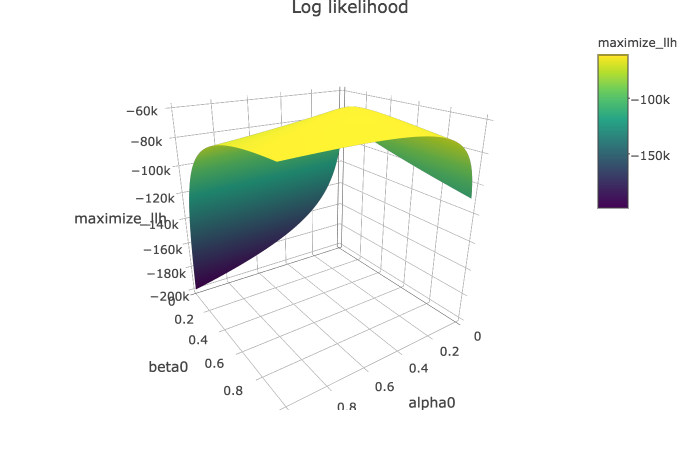
\includegraphics[width=1\textwidth]{./figures/loglikelihood.png}
	\caption{Log likelihood function of the dataset related to the first product. The maximum is found at $\alpha = 0.52$ and $\beta = 0.82$}
	\label{fig:loglikelihood}
\end{figure}

\subsection{Quality of the model}

In order to judge the quality of the model, in the table below, we present the error between the model and data as a percentage. We observe that the model trained on the full data agrees better with the date than the model used for prediction, with a maximum deviation of $10\%$ vs $~40\%$. Overall, the predictive model overestimates the survival probability, which, when known, could be manually corrected by using knowledge of historical data. 

\begin{figure*}[t!]
	\centering
	\begin{subfigure}[b]{0.5\textwidth}
		\centering
		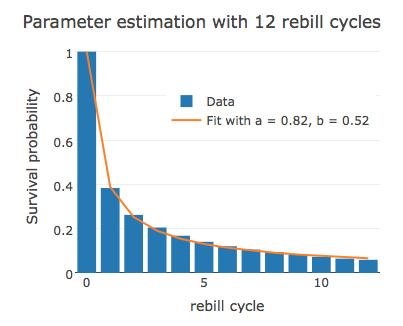
\includegraphics[height=2.1in]{./figures/VR12cycles.png}
		\caption{Model trained on full data set.}
	\end{subfigure}%
	~ 
	\begin{subfigure}[b]{0.5\textwidth}
		\centering
		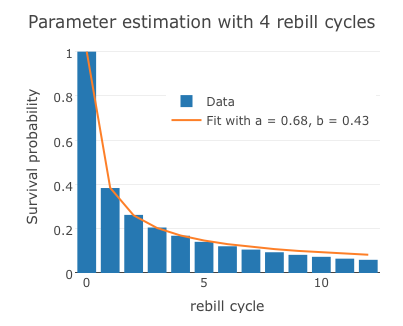
\includegraphics[height=2.1in]{./figures/VR4cycles.png}
		\caption{Model trained on partial data set.}
	\end{subfigure}
	\caption{Data and modelling for the first product considered.}
	\label{Frobenius}
\end{figure*}

\begin{table}[ht]
	\centering
	\begin{tabular}{rrrr}
		\hline
		\multicolumn{2}{c|}{12 cycles for parameter estimation} & \multicolumn{2}{c}{4 cycles for parameter estimation} \\
		\hline
		Rebill cycle & Error (\%) & Rebill cycle &  Error (\%) \\ 
		\hline
		0 & 0.00 & 0 & 0.00\\ 
		1 & 1.31 & 1 & 0.24\\ 
		2 & -3.70 & 2 & -0.85 \\ 
		3 & -7.13 & 3 & -1.12 \\ 
		4 & -8.02 & 4 & 0.66 \\ 
		5 & -6.90 & 5 & 4.26 \\ 
		6 & -5.47 & 6 & 8.00 \\ 
		7 & -4.13 & 7 & 11.45  \\ 
		8 & -2.43 & 8 & 15.19 \\ 
		9 & 1.70 & 9 & 21.74  \\ 
		10 & 5.13 & 10 & 27.44  \\ 
		11 & 10.05 & 11 & 34.96 \\ 
		12 & 11.67 & 12 & 38.41 \\ 
		\hline
	\end{tabular}
	\caption{Errors between data and model for first product, where two left most column quantify error for model trained on full dataset, and two left most column on partial dataset.}
	\label{VR}
\end{table}

We repeat the same type of analysis for a second product

\begin{figure*}[t!]
	\centering
	\begin{subfigure}[b]{0.5\textwidth}
		\centering
		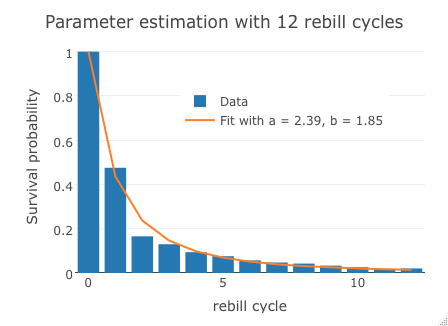
\includegraphics[height=2.1in]{./figures/SV12cycles.png}
		\caption{Model trained on full data set.}
	\end{subfigure}%
	~ 
	\begin{subfigure}[b]{0.5\textwidth}
		\centering
		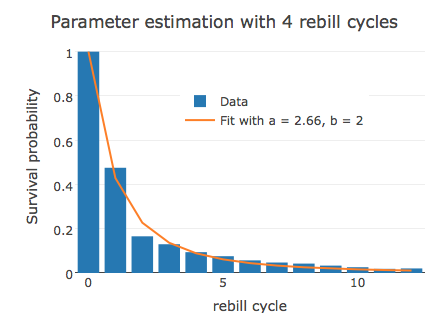
\includegraphics[height=2.1in]{./figures/SV4cycles.png}
		\caption{Model trained on partial data set.}
	\end{subfigure}
	\caption{Data and modelling for the second product considered.}
	\label{Frobenius}
\end{figure*}


\begin{table}[ht]
	\centering
	\begin{tabular}{rrrr}
		\hline
		\multicolumn{2}{c|}{12 cycles for parameter estimation} & \multicolumn{2}{c}{4 cycles for parameter estimation} \\
		\hline
		Rebill cycle & Error (\%) & Rebill cycle &  Error (\%) \\ 
		\hline
		0 & 0.00 & 0 & 0.00\\ 
		1 & -8.28 & 1 & -9.78\\ 
		2 & 43.01 & 2 & 37.09 \\ 
		3 & 12.51 & 3 & 4.99 \\ 
		4 & 4.02 & 4 & -5.41\\ 
		5 & -8.46 & 5 & -18.77 \\ 
		6 & -9.78 & 6 & -21.74 \\ 
		7 & -16.68 & 7 & -29.24  \\ 
		8 & -26.92 & 8 & -39.16 \\ 
		9 & -25.16 & 9 & -38.85 \\ 
		10 & -21.58 & 10 & -37.03 \\ 
		11 & -9.49 & 11 & -28.51 \\ 
		12 & -30.43 & 12 & -45.90 \\ 
		\hline
	\end{tabular}
	\caption{Errors between data and model for second product, where two left most column quantify error for model trained on full dataset, and two left most column on partial dataset.}
	\label{SV}
\end{table}



\begin{thebibliography}{9}
	
	\bibitem{feder07}
	Peter S. Fader and Bruce G. S. Hardie
	\textit{ How To Project Customer
		Retention},
	2007.
	
	\bibitem{feder09}
	Peter S. Fader and Bruce G. S. Hardie
	\textit{ Probability Models for Customer-Base Analysis},
	2009.
	
\end{thebibliography}
\end{document}